\documentclass[17pt, t, lualatex]{beamer}



\title{\LARGE Cambio en los Ingresos de Familias Desplazadas del Meta por el Conflicto Armado}
\date{\today}
\institute[UJTL]{Universidad Jorge Tadeo Lozano}
\author{Ludwig Alvarado Becerra}

\usepackage{amsmath, amssymb, mathtools}
\usepackage[spanish]{babel}
\usepackage{biblatex}
\usepackage{hyperref}
\usepackage{xurl}
\usepackage{cancel}
\usepackage{svg}

\addbibresource{referencias.bib}  % Make sure your .bib file is correctly named


\addbibresource{referencias.bib}

% Probably load as late as possible
% Other options are
% - engine=pdflatex to compile in pdfLaTeX (with different fonts),
% - mathshape=rm to use serif font for math,
% - mathsahpe=custom to not set any math font (so that you can define your own math fonts)
\usetheme[engine=lualatex, mathshape=sf, fontdir=kthpq-files/fonts/Figtree/]{kthpq}
\setmonofont{Bitstream Vera Sans Mono}[Scale=.9]

% Custom colors (see beamercolorthemecustom.sty for more details)
% \usecolortheme{custom}

% Modify the headline template: KTH-full, KTH-section-only, or KTH-frametitle-only.
% \setbeamertemplate{headline}[KTH-full]

% Custom footline
% \setfootline{left}{center}{right}

\begin{document}

\inserttitlepage

\section{Hallazgos \textit{papers}}

\insertsectionpage

\begin{frame}[allowframebreaks]
  \frametitle{Hallazgos \textit{papers}}
  Se consultaron principalmente los siguientes artículos científicos:
  \begin{itemize}
    \item \textit{Predicting forced displacement using a generalised and automated agentbased simulation} \cite{suleimenova2020predicting}
    \item \textit{An agent-based model to identify migration pathways of refugees: the case of syria} \cite{hebert2017agent}
    \item \textit{Teorı́a de la migración colectiva como explicación al desplazamiento forzado en colombia} \cite{Gutierrez2012}
    \item \textit{Importancia de la economı́a campesina en los contextos contemporáneos: una mirada al caso colombiano}\cite{santacoloma2015importancia}
    \item \textit{Impacto económico de la violencia armada sobre la producción campesina, caso municipios zona de distensión departamento del meta, colombia (1991-2014)} \cite{perez2016impacto}
  \end{itemize}

\end{frame}

\section{Predicting forced displacement using a generalised and automated
  agentbased simulation}


\insertsectionpage

\begin{frame}[allowframebreaks]
  \frametitle{Hallazgos \textit{papers}}
  
  \begin{columns}
    \begin{column}{.5\textwidth}
      \begin{itemize}
        \item Aplican ABM para Burundi, República Centroafricana y Mali.
        \item Predicen la distribución de migrantes en los campos.
        \item Utilizan FLEE\cite{groen_flee_2023} y
              FabSim3\cite{groen_fabsim3_2023}.
        \item Aplican el modelo a una escala grande.
      \end{itemize}
    \end{column}

    \begin{column}{.5\textwidth}
      \begin{figure}[ht]
        \centering
        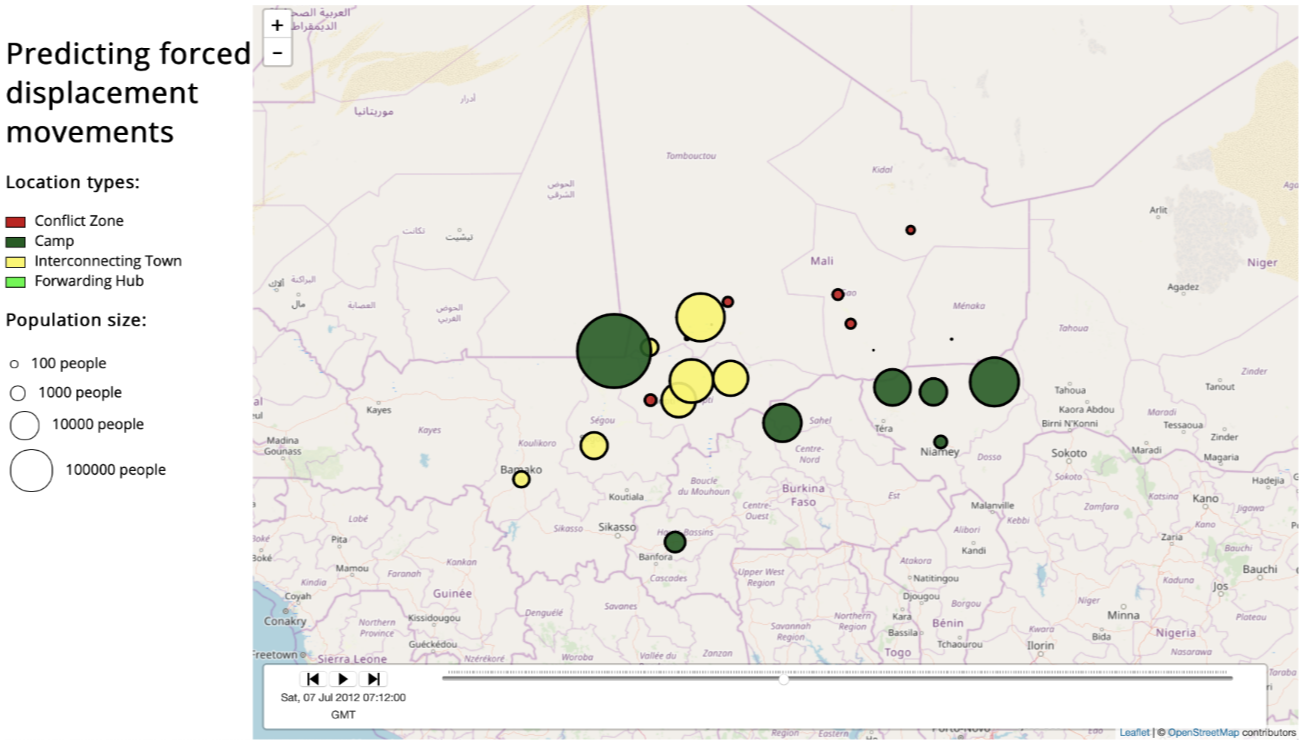
\includegraphics[width=0.8\textwidth]{img/Paper2Fig1.png}
        \caption{\label{fig:p1f1} Salida de la simulación usando VisualFlee\cite{Visualflee,suleimenova2020predicting}}
      \end{figure}

    \end{column}
  \end{columns}

\end{frame}



\section{An Agent - Based Model to Identify Migration Pathways of Refugees: The
  Case of Syria}

\insertsectionpage

\begin{frame}[allowframebreaks]
  \frametitle{Hallazgos \textit{papers}}
  
  \begin{columns}
    \begin{column}{.5\textwidth}
      \begin{itemize}
        \item El modelo propone patrones de migración de Siria.
        \item Proponen una decisión para irse. (Tolerancia)
        \item Elección de destinación por medio de diferentes condicionales.
        \item Muestran la simulación con datos geoespaciales de Bing.
      \end{itemize}
    \end{column}

    \begin{column}{.5\textwidth}
      \begin{figure}[ht]
        \centering
        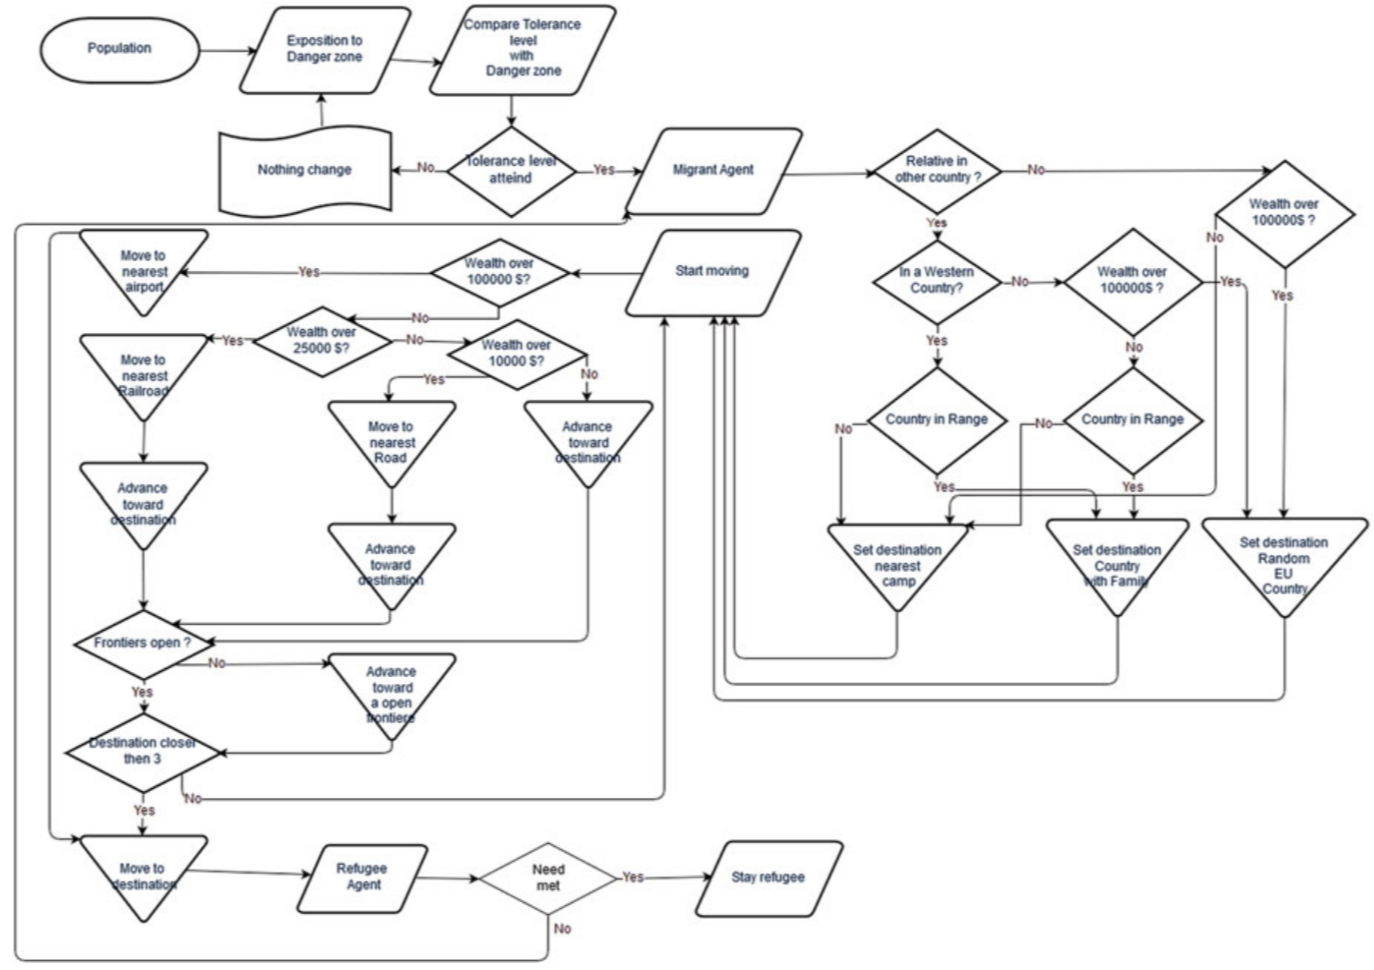
\includegraphics[width=0.7\textwidth]{img/Paper1Fig1.png}
        \caption{\label{fig:p1f1} Diagrama de flujo para el modelo.\cite{suleimenova2020predicting}}
      \end{figure}

    \end{column}
  \end{columns}

\end{frame}

\section{Teorı́a de la migración colectiva como explicación al desplazamiento forzado en colombia}

\insertsectionpage

\begin{frame}[allowframebreaks]
  \frametitle{Hallazgos \textit{papers}}
  
  \begin{columns}
    \begin{column}{.5\textwidth}
      \begin{itemize}
        \item Aplican ABM en el conflicto en Colombia por medio de la teoría de
              migración colectiva.
        \item La decisión individual de migración afecta a la migración colectiva.
        \item Los individuos sin ninguna relación transfieren información al
              grupo de manera emergente.
      \end{itemize}
    \end{column}

    \begin{column}{.5\textwidth}
      \begin{figure}[ht]
        \centering
        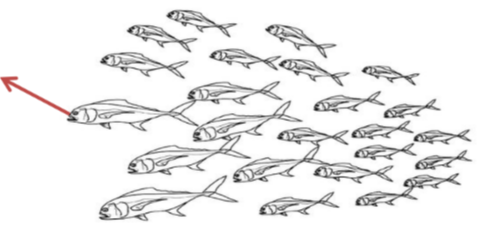
\includegraphics[width=0.7\textwidth]{img/Paper3Fig1.png}
        \caption{\label{fig:p1f1} Comportamiento animal colectivo\cite{Gutierrez2012}}
      \end{figure}

    \end{column}
  \end{columns}

\end{frame}

\section{Importancia de la economı́a campesina en los contextos contemporáneos: una mirada al caso colombiano}

\insertsectionpage

\begin{frame}[allowframebreaks]
  \frametitle{Hallazgos \textit{papers}}
  
  \begin{columns}
    \begin{column}{.5\textwidth}
      \begin{itemize}
        \item Las economías campesinas permiten la biodiversidad genética,
              abastecimiento de alimentos en zonas apartadas, consolidación de
              mercados locales y redes de cooperación en zonas rurales.              
        \item La agricultura campesina es bastante eficiente y no aplica
              principios empresariales.
        \item Abandono estatal ocasionando pobreza.
      \end{itemize}
    \end{column}

    \begin{column}{.5\textwidth}
      \begin{figure}[ht]
        \centering
        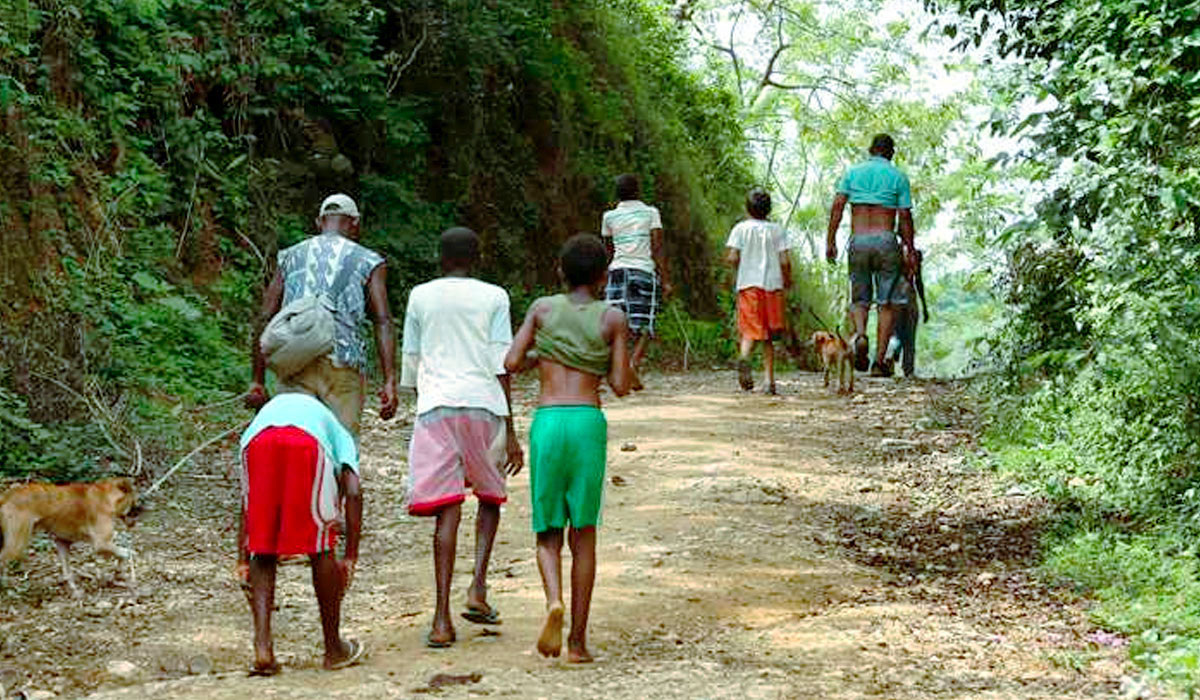
\includegraphics[width=0.7\textwidth]{img/Paper4Fig1.png}
        \caption{\label{fig:p1f1} Imagen sacada de FarodiRoma\cite{farodiroma_choco_2025}}
      \end{figure}

    \end{column}
  \end{columns}

\end{frame}

\section{Impacto económico de la violencia armada sobre la producción campesina,
  caso municipios zona de distensión departamento del Meta, Colombia (1991-2014)}

\insertsectionpage

\begin{frame}[allowframebreaks]
  \frametitle{Hallazgos \textit{papers}}
  
  \begin{columns}
    \begin{column}{.5\textwidth}
      \begin{itemize}
        \item Recolectan datos de la producción agrícola de los campesinos y
              cómo se afectan con el conflicto armado.              
        \item Realizan modelos para estimar la cantidades producidas de un
              producto y ver cómo se ven afectadas al ingresar un grupo armado.
        \item Concluyen con una confianza del 99\% que el desplazamiento explica
              la producción de diferentes productos campesinos y es importante
              en el modelo.
      \end{itemize}
    \end{column}

    \begin{column}{.5\textwidth}
      \begin{figure}[ht]
        \centering
        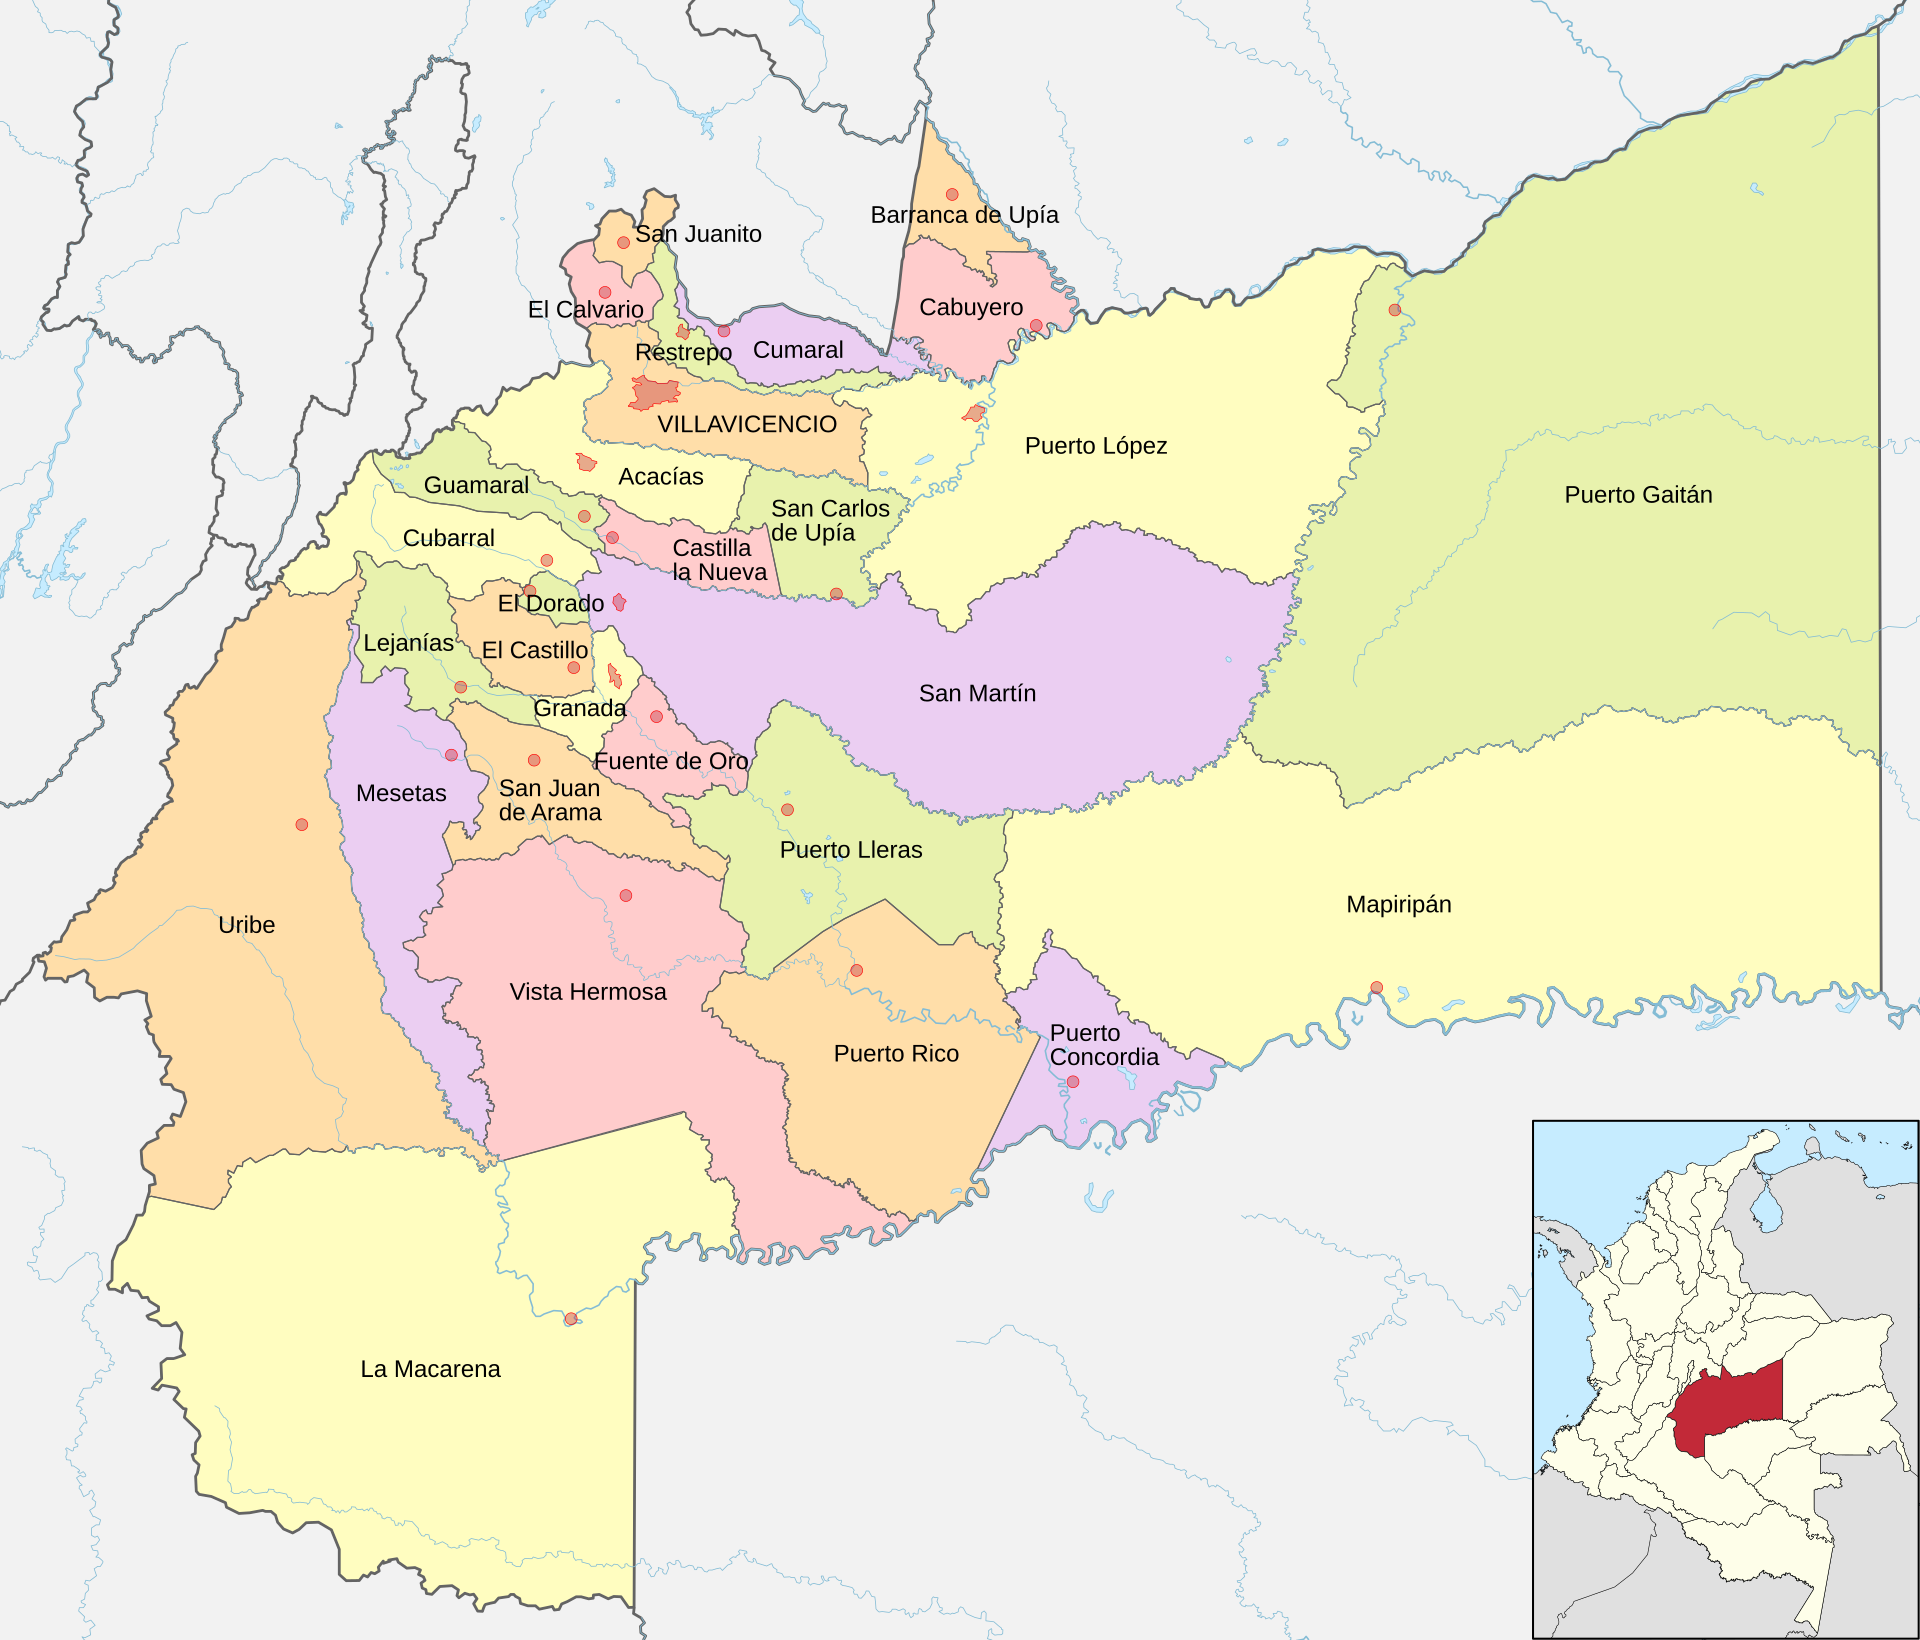
\includegraphics[width=0.7\textwidth]{img/MapaMeta.png}
        \caption{\label{fig:p1f1} Mapa político del Meta \cite{eswiki:166396423}}
      \end{figure}

    \end{column}
  \end{columns}

\end{frame}


\section{Ideas}

\insertsectionpage


\begin{frame}[allowframebreaks]
  \frametitle{Hallazgos \textit{papers}}
  Principales ideas
  \begin{itemize}
    \item Dos agentes: campesinos y grupo armado.
    \item Valor de violencia percibida por la población campesina.
    \item Atributo para campesinos: \texttt{Desplazado} \texttt{No desplazado}.
    \item Campesinos atributo de tolerancia al peligro.
    \item Campesinos con métodos para generar ingresos.
    \item Agregar aleatoriedad a los métodos de generar ingresos.
  \end{itemize}
\end{frame}

\begin{frame}[allowframebreaks]
  \frametitle{Hallazgos \textit{papers}}
  
  Valoración ambiental del Meta\cite{EVA2020}, principales producciones de cultivos (2020):
  
  \begin{itemize}
    \item Aguacate $35014.28\ t$ 
    \item Caña azucarera $56170.40\ t$
    \item Cítricos $76298.28\ t$
    \item Maracuyá $44967.31\ t$
    \item Palma de aceite $637606.60\ t$
    \item Piña $116775.02\ t$
    \item Plátano $396613.49\ t$
  \end{itemize}


\end{frame}

\begin{frame}[allowframebreaks]
  \frametitle{Métodos para ingresos de los campesinos}
  

  \begin{itemize}
    \item Se va a asumir que todos los campesinos producen lo mismo en mismas cantidades y únicamente cultivos. 
    \item Función \texttt{producir\_\{\textit{cultivo}\}(\textit{int}):\textit{float}}.
    \item Se resta el costo de producción promedio de cada cultivo.
    \item Se utilizan cuando la condición del agente es \texttt{no migrante}.
  \end{itemize}


\end{frame}

\begin{frame}[allowframebreaks]
  \frametitle{Ejemplo producción aguacate}
  
  \begin{itemize}
    \item Campesinos (registrados) en el Meta: $16211$\cite{EVA2020}
    \item Producción de aguacate: $35014.28\ t/a$\cite{EVA2020}
    \item Valor aguacate: $2915.5\ \$/kg$\cite{CifrasSectoriales2021}
    \item Costo producción aguacate: $879 \$/kg$\cite{Finagro2022}
  \end{itemize}

\end{frame}

\begin{frame}[allowframebreaks]

  Se desea que todo esté en valores de peso por día $\$/d$.

\end{frame}


\begin{frame}[allowframebreaks]

  Se desea que todo esté en valores de peso por día $\$/d$.

    \[
    \frac{35014.28\ \cancel{t}}{1\  \cancel{\text{año}}} \times \left( \frac{1 \  \cancel{\text{año}}}{365 \ \text{días}}  \right) \times \left( \frac{1000\ kg}{1 \ \cancel{t}} \right)
    \]

\end{frame}


\begin{frame}[allowframebreaks]

  Se desea que todo esté en valores de peso por día $\$/d$.

    \[
    \frac{35014.28\ \cancel{t}}{1\  \cancel{\text{año}}} \times \left( \frac{1 \  \cancel{\text{año}}}{365 \ \text{días}}  \right) \times \left( \frac{1000\ kg}{1 \ \cancel{t}} \right)
  \]

  \[
    95929.53 \frac{kg}{\text{día}} \times \left( \frac{1}{16211}\right) = 5.92 \frac{kg}{\text{día}} 
  \]

\end{frame}


\begin{frame}[allowframebreaks]

  Se desea que todo esté en valores de peso por día $\$/d$.

    \[
    \frac{35014.28\ \cancel{t}}{1\  \cancel{\text{año}}} \times \left( \frac{1 \  \cancel{\text{año}}}{365 \ \text{días}}  \right) \times \left( \frac{1000\ kg}{1 \ \cancel{t}} \right)
  \]

  \[
    95929.53 \frac{kg}{\text{día}} \times \left( \frac{1}{16211}\right) = 5.92 \frac{kg}{\text{día}} 
  \]

  \[
    \left(2912.5 \frac{\$}{\cancel{kg}} - 879 \frac{\$}{\cancel{kg}} \right) \times 5.92 \frac{\cancel{kg}}{\text{día}} = 12038.32 \frac{\$}{\text{día}}
  \]

\end{frame}


\begin{frame}
  \begin{itemize}
    \item Un campesino en promedio gana $12032.32$ pesos al día por su producción de aguacate.
    \item Repetir el proceso con lo demás métodos.
    \item Se contempleta agregar una incertidumbre para la variabilidad de cada campesino.
  \end{itemize}
\end{frame}

\begin{frame}
  \frametitle{Clase Campesino}
  \begin{figure}[ht]
    \centering
    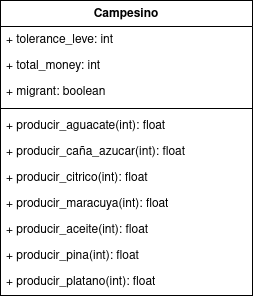
\includegraphics[width = 0.3\textwidth]{img/Migraciones.png}
  \end{figure}

\end{frame}


\section{Licencia proyecto}

\insertsectionpage


\begin{frame}
  \frametitle{Licencia}

\begin{columns}
  \begin{column}{.5\textwidth}
    \begin{itemize}
      \item El código está bajo una licencia GPL V3, las presentaciones y escritos bajo la CC 4.0
      \item Todo el proyecto (bibliografía, avances, presentaciones y código) se encuentra en el siguiente enlace a \textit{GitHub} \url{https://github.com/TheLudway/abm-forced-displacement}
    \end{itemize}
  \end{column}

  \begin{column}{.5\textwidth}
    \begin{figure}[ht]
      \centering
      
\includegraphics[width = 0.7\textwidth]{img/gpl.png}
    \end{figure}

  \end{column}
\end{columns}


\end{frame}




\section{Referencias}

\insertsectionpage
\begin{frame}[allowframebreaks]{Referencias}
  \printbibliography
\end{frame}


\insertendpage

\end{document}
